\documentclass[a4paper,14pt]{extreport} % формат документа

\usepackage{amsmath}
\usepackage{cmap} % поиск в ПДФ
\usepackage[T2A]{fontenc} % кодировка
\usepackage[utf8]{inputenc} % кодировка исходного текста
\usepackage[english,russian]{babel} % локализация и переносы
\usepackage[left = 2cm, right = 1cm, top = 2cm, bottom = 2 cm]{geometry} % поля
\usepackage{listings}
\usepackage{graphicx} % для вставки рисунков
\usepackage{amsmath}
\usepackage{float}
\usepackage{multirow}
\graphicspath{{pictures/}}
\DeclareGraphicsExtensions{.pdf,.png,.jpg}
\newcommand{\anonsection}[1]{\section*{#1}\addcontentsline{toc}{section}{#1}}

\lstset{ %
	language=Prolog,                % Язык программирования 
	numbers=left,                   % С какой стороны нумеровать          
	frame=single,                    % Добавить рамку
}

\begin{document}
\begin{titlepage}

    \begin{table}[H]
        \centering
        \footnotesize
        \begin{tabular}{cc}
            \multirow{8}{*}{
\includegraphics[scale=0.35]{bmstu.jpg}}
            & \\
            & \\
            & \textbf{Министерство науки и высшего образования Российской Федерации} \\
            & \textbf{Федеральное государственное бюджетное образовательное учреждение} \\
            & \textbf{высшего образования} \\
            & \textbf{<<Московский государственный технический} \\
            & \textbf{университет имени Н.Э. Баумана>>} \\
            & \textbf{(МГТУ им. Н.Э. Баумана)} \\
        \end{tabular}
    \end{table}

    \vspace{-2.5cm}

    \begin{flushleft}
        \rule[-1cm]{\textwidth}{3pt}
        \rule{\textwidth}{1pt}
    \end{flushleft}

    \begin{flushleft}
        \small
        ФАКУЛЬТЕТ
        \underline{<<Информатика и системы управления>>\ \ \ \ \ \ \ 
        \ \ \ \ \ \ \ \ \ \ \ \ \ \ \ \ \ \ \ \ \ \ \ \ \ \ \ \ \ \ \ 
    \ \ \ \ \ \ \ \ \ \ \ \ \ \ \ } \\
        КАФЕДРА
        \underline{<<Программное обеспечение ЭВМ и
        информационные технологии>>
        \ \ \ \ \ \ \ \ \ \ \ \ \ \ \ \ \ \ \ \ }
    \end{flushleft}

    \vspace{4cm}

    \begin{center}
        \textbf{Лабораторная работа № 11} \\ 
        \hfill
        
        \textbf{Среда Visual Prolog 5.2} \\
        \vspace{0.5cm}
        \textbf{} \\
    \end{center}

    \vspace{4cm}

    \begin{flushleft}
        \begin{tabular}{ll}
            \textbf{Дисциплина} & Функциональное и логическое программирование \\
            \textbf{Студент} & Сиденко А.Г. \\
            \textbf{Группа} & ИУ7-63Б \\
            \textbf{Преподаватель} & Толпинская Н.Б., Строганов Ю.В.  \\
        \end{tabular}
    \end{flushleft}

    \vspace{4cm}

   \begin{center}
        Москва, 2020 г.
    \end{center}

\end{titlepage}

\textbf{Задание}

Запустить среду Visual Prolog5.2. Настроить утилиту TestGoal. Запустить тестовую программу, проанализировать реакцию системы и множество ответов. Разработать свою программу -- <<Телефонный справочник>>. Протестировать работу программы. 

\textbf{Программа <<Телефонный справочник>>}

\begin{lstlisting}
predicates
  abonent(string, string).
clauses
  abonent(ellen, "111111").
  abonent(ellen, "777777").
  abonent(john, "222222").
  abonent(tom, "333333").
  abonent(eric, "444444").
  abonent(eric, "888888").
  abonent(eric, "999999").
  abonent(mark, "555555").
  abonent(bill, "666666").
goal
  Name = mark,
  write(Name, " numbers: "), nl,
  abonent(Name, Number).
\end{lstlisting}

\textbf{Примеры работы}

\begin{enumerate}
\item Если имени нет в телефонной книге


\includegraphics{ex1}

\item Если имя встречается один раз в телефонной книге

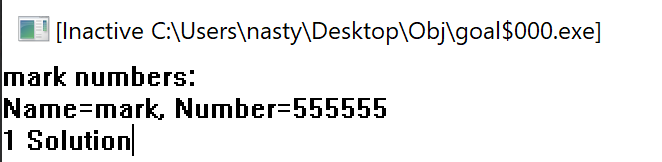
\includegraphics{ex2}

\newpage

\item Если имя встречается несколько раз в телефонной книге

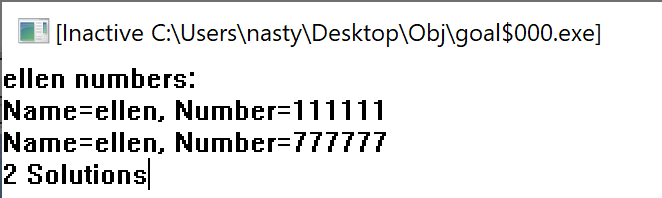
\includegraphics{ex3}
\end{enumerate}

\textbf{Ответы на вопросы}

что собой представляет программа на Prolog, какова ее структура. Как она реализуется, как формируются результаты работы программы. 

\textbf{Программа на Prolog представляет собой:} базу знаний и вопрос. База знаний содержит истинностные знания, используя которые программа выдает ответ на запрос. 

Основным элементом языка является терм. Терм – это: константа, переменная, составной терм. С помощью термов и более сложных конструкций языка Prolog – фактов и правил <<описываются>> знания о предметной области, т.е. база знаний. Используя базу знаний, система Prolog будет делать логические выводы, отвечая на наши вопросы. 

Программа на Prolog состоит из разделов. Каждый раздел начинается со своего заголовка. 

\textbf{Структура программы }
\begin{enumerate}
\item директивы компилятора -- зарезервированные символьные константы
\item CONSTANTS -- раздел описания констант
\item DOMAINS -- раздел описания доменов
\item DATABASE -- раздел описания предикатов внутренней базы данных
\item PREDICATES -- раздел описания предикатов
\item CLAUSES -- раздел описания предложений базы знаний
\item GOAL -- раздел описания внутренней цели (вопроса).
\end{enumerate}

В программе не обязательно должны быть все разделы.

С помощью подбора ответов на запросы он (Prolog, программа) извлекает хранящуюся (известную в программе) информацию. Одной из особенностей Prolog является то, что при поиске ответов на вопрос, он рассматривает альтернативные варианты и находит все возможные решения (методом проб и ошибок) -- множества значений переменных, при которых на поставленный вопрос можно ответить -- <<да>>.

Поиск содержательного ответа на поставленный вопрос, с помощью имеющейся базы знаний, фактически заключается в поиске нужного знания, но какое знание понадобится – заранее неизвестно. Этот поиск осуществляется формально с помощью механизма унификации. Упрощенно, процесс унификации можно представить как формальный процесс сравнивания терма вопроса с очередным термом знания. При этом, знания по умолчанию просматриваются сверху вниз. В процессе сравнивания для переменных «подбираются», исходя из базы знаний, значения или подтверждается истинность вопроса. 

\end{document}